\documentclass[12pt,letterpaper]{report}
\usepackage{pgf, tikz}
\usetikzlibrary{arrows, automata}
\usepackage{graphicx}
\usepackage{hyperref}
\usepackage{xcolor}
\usepackage{caption}

\begin{document}
\begin{titlepage}
\begin{center}


\includegraphics{C:/Users/User/Pictures/bsmrstu.jpg}\\
[0.4cm]
\textsc{\huge Bangabandhu Sheikh Mujibur Rahman Science and}
\textsc{\huge  Technology University }
\linebreak
\textit{\large { \color{purple} (SHIICT)}} \\
\line (1,0) {320}\\
[0.6cm]

\textsc{\huge {\color{blue}T}{\color{magenta}HE GRAPH THEORY}}\\
[0.3cm]
\line (1,0) {250}\\
[0.1cm]
\textit{\large A{ \color{red} \LaTeX}  Report}\\
[1.3cm]
\textbf{\huge \color{teal}  Authored By:}\\
[0.7cm]
{\huge Name : Anisur Rahaman}\\
{\Large Session : 2018-2019}\\
\Large ID : 18ICTCSE017\\
\textsc{\Large Department Of : Computer Science and Engineering}\\
[1cm]
\color{blue}
22 January, 2020\\
\end{center}
\end{titlepage}
\newpage
{\color{teal}\tableofcontents
\pagenumbering{roman}}

\begin{center}

\end{center}
 \chapter{}
\pagenumbering{roman}
\section{Introduction}\label{sec:intro}

 Graph is a {\textbf{mathematical representation of a network} mathematical representation of a network} and it describes the relationship between lines and points. A graph consists of some points and lines between them. The length of the lines and position of the points do not matter. Each object in a graph is called a node.\\
[0.8cm]
Graph theory can play vital role directly or indirectly in our practical life.it's used in many ways to determine shortest path among the different ways.Basically, it's uses at a high extent in all plateform.For example, 
computer science,physics and chemistry,Biology,Mathematics,Social Science etc. \\
[0.8cm]
So, i will try to delineate as well as politely describe my document about Graph Theory what i illustrated in next phage with the help of Wikipedia and related to several website about the Graph  theory.
 
\chapter{}
\begin{center}
\textsc{\Huge {\color{blue}T}{\color{magenta}HE GRAPH THEORY}}\\
\end{center}
\section{definition: }


 {\Huge \color{red}G}raphs are discrete structures consisting of vertices and edges that connect these vertices.
There are different kinds of graphs, depending on whether edges have directions, whether
multiple edges can connect the same pair of vertices, and whether loops are allowed. Problems
in almost every conceivable discipline can be solved using graph models.We will give examples
to illustrate how graphs are used as models in a variety of areas. For instance, we will show how
graphs are used to represent the competition of different species in an ecological niche, how
graphs are used to represent who influences whom in an organization, and how graphs are used
to represent the outcomes of round-robin tournaments.\\
[0.7cm]

\subsection{Types of Graphs : }
\begin{enumerate}
{\color{orange}{\large \item Null graph:}} Also called an empty graph, a null graph is a graph in which there are no edges between any of its vertices.
{\color{orange}{\large \item Connected graph :}}A graph in which there is a path of edges between every pair of vertices in the graph. Mary's graph is a connected graph, since there is a way to get from every city on the map to every other city.
{\color{orange}{\large \item Disconnected graph :}}A graph in which the path of edges does not always connect every vertex.
{\color{orange}{\large \item Bipartite graph: }}A graph that can be split into two sets of vertices such that edges only go between sets, not within them.
{\color{orange}{\large \item Weighted graph: }}A graph in which weights, or numerical values, are assigned to each of the edges. Mary's graph is a weighted graph, where the distances between the cities are the weights of the edges.
{\color{orange}{\large \item Directed graph: }}A graph in which the edges are directed by arrows, indicating that the relationship, represented by the edge, only applies from one vertex to the other, but not the other way around. In other words, if a directed edge has an arrow from A to B, A is related to B, but B is not related to A.
{\color{orange}{\large \item Undirected graph:} }A graph whose edges are not directed. Mary's graph is an undirected graph, because the routes between cities go both ways.
{\color{orange}{\large \item Simple graph:}}An undirected graph in which there is at most one edge between each pair of vertices, and there are no loops, which is an edge from a vertex to itself.
{\color{orange}{\large \item Multi-graph: }}A graph in which there are multiple edges between any pair of vertices or there are edges from a vertex to itself, also called a loop.
{\color{orange}{\large \item Planar graph: }}A graph that can be drawn so that all of the edges of the graph do not cross each other.
 
\newpage
\section{graph Details:}
\subsection{{\color{blue}Directed Graph :}}A directed graph (or digraph) (V, E) consists of a nonempty set of vertices set of
directed edges (or arcs) E. Each directed edge is associated with an ordered pair of vertices.
The directed edge associated with the ordered pair (u, v) is said to start at u and end at v.There have also weight of every nodes respectively.Foe example,v1 to s node is 18,s v2 node is 1 etc.
\end{enumerate}
\begin{center}
    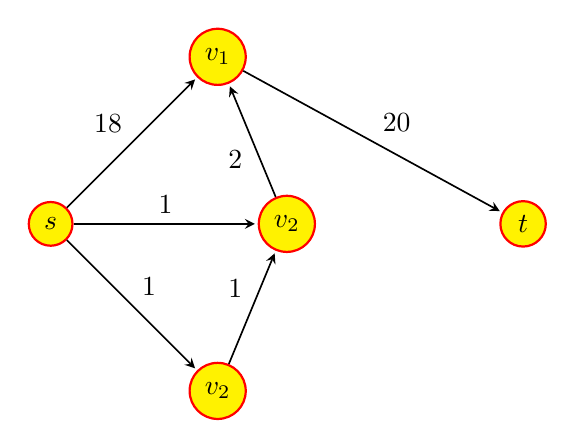
\begin{tikzpicture}[
            > = stealth, 
            shorten > = 1pt,
            auto,
            node distance = 3cm, 
            semithick 
        ]

        \tikzstyle{every state}=[
            draw =red,
            thick,
            fill = yellow,
            minimum size = 4mm
        ]
        \node[state] (s) {$s$};
        \node[state] (v1) [above right of=s] {$v_1$};
        \node[state] (v2) [right of=s] {$v_2$};
        \node[state] (v3) [below right of=s] {$v_2$};
        \node[state] (t) [right of=v2] {$t$};

        \path[->] (s) edge node {18} (v1);
        \path[->] (s) edge node {1} (v2);
        \path[->] (s) edge node {1} (v3);
        \path[->] (v2) edge node {2} (v1);
        \path[->] (v3) edge node {1} (v2);
        \path[->] (v1) edge node {20} (t);

        \draw[red, dashed] (1, 2) (1, -2);
    \end{tikzpicture}
 
    \end{center}
\subsection{{\color{blue}Bipartite Graph :}} A bipartite graph ‘G’, G = (V, E) with partition V = {V1, V2} is said to be a complete bipartite graph if every vertex in V1 is connected to every vertex of V2.

In general, a complete bipartite graph connects each vertex from set V1 to each vertex from set V2.\\

\large Example : \\
The following graph is a complete bipartite graph because it has edges connecting each vertex from set V1 to each vertex from set V2.
\begin{center}
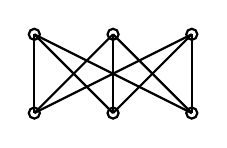
\begin{tikzpicture}[style=thick]
\foreach \x in {0,1,2}
\foreach \y in {0,1,2}
{\draw (\y,1) -- (\x,2);}
\foreach \x in {0,1,2}{
\draw (\x,1) circle (2pt);
\draw (\x,2) circle (2pt);}
\end{tikzpicture}
\subsection{{\color{blue}Undirected Graph :}}An undirected graph is graph, i.e., a set of objects (called vertices or nodes) that are connected together, where all the edges are bidirectional. An undirected graph is sometimes called an undirected network. In contrast, a graph where the edges point in a direction is called a directed graph.

When drawing an undirected graph, the edges are typically drawn as lines between pairs of nodes, as illustrated in the following figure.

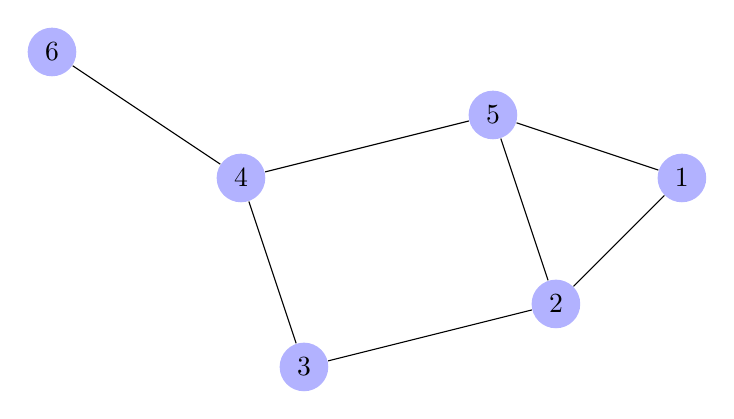
\begin{tikzpicture}
  [scale=.8,auto=left,every node/.style={circle,fill=blue!30}]
  \node (n6) at (1,10) {6};
  \node (n4) at (4,8)  {4};
  \node (n5) at (8,9)  {5};
  \node (n1) at (11,8) {1};
  \node (n2) at (9,6)  {2};
  \node (n3) at (5,5)  {3};

  \foreach \from/\to in {n6/n4,n4/n5,n5/n1,n1/n2,n2/n5,n2/n3,n3/n4}
    \draw (\from) -- (\to);

\end{tikzpicture}
\end{center}
\newpage
\chapter{\color{blue}{}History of Graph theory :}
\section{Father of Graph Theory :}
\includegraphics[height=5cm]{C:/Users/User/Pictures/Frank Harary.jpg}\\
{\huge Frank Harary :} \\
{{\color{red}\textbf{Frank Harary :} }(March 11, 1921 – January 4, 2005) was an American mathematician, who specialized in {\textbf{graph theory.}} He was widely recognized as one of the "fathers" of modern graph theory. Harary was a master of clear exposition and, together with his many doctoral students, he standardized the terminology of graphs. He broadened the reach of this field to include physics, psychology, sociology, and even anthropology. Gifted with a keen sense of humor, Harary challenged and entertained audiences at all levels of mathematical sophistication. A particular trick he employed was to turn theorems into games - for instance, students would try to add red edges to a graph on six vertices in order to create a red triangle, while another group of students tried to add edges to create a blue triangle (and each edge of the graph had to be either blue or red). Because of the theorem on friends and strangers, one team or the other would have to win.

Frank Harary was born in New York City, the oldest child to a family of Jewish immigrants from Syria and Russia. He earned his bachelor's and master's degrees from Brooklyn College in 1941 and 1945 respectively and his Ph.D., with supervisor Alfred L. Foster, from University of California, Berkeley in 1948.

Prior to his teaching career he became a research assistant in the Institute of Social Research at the University of Michigan.
\subsection{{\color{blue} Biography :}}
{\Huge \color{cyan}H}arary's first publication, {\color{red}\textit{"Atomic Boolean-like rings with finite radical"} }, went through much effort to be put into the Duke Mathematical Journal in 1950. This article was first submitted to the American Mathematical Society in November 1948, then sent to the Duke Mathematical Journal where it was revised three times before it was finally published two years after its initial submission.[citation needed] Harary began his teaching career at the University of Michigan in 1953 where he was first an assistant professor, then in 1959 associate professor and in 1964 was appointed as a professor of mathematics, a position he held until 1986.\\
\newpage
\subsection{{\color{blue} The Birth of Graph Theory:}}{\Huge \color{magenta}T}he good people of {\color{green}\textit{"Königsberg"} }, Germany (now a part of Russia), had a puzzle that they liked to contemplate while on their Sunday afternoon walks through the village. The Preger River completely surrounded the central part of Königsberg, dividing it into two islands. These islands were connected to each other and to the mainland by seven bridges. The puzzle, which baffled the residents of Königsberg was this: Was it possible to pick a starting point in the town and find a walking route which would take them over each bridge exactly once? No one had ever found such a route; but did that mean that it did not exist? The problem caught the attention of the great Swiss mathematician, Leonhard Euler. Euler was able to prove that such a route did not exist, and in the process began the study of what was to be called graph theory.
\begin{figure}
\centering 
\includegraphics[height=5cm]{C:/Users/User/Pictures/bridge of konigsberg.jpg}\\
\caption{Bridge of Kingston }
\end{figure}
  
\newpage
\chapter{Application}
\section{Several Application}
\subsection{{\color{teal}The Cantor-Schröder-Bernstein Theorem:}}Here we discuss the graph theoretical proof of the classical result of Schröder and Bernstein. This theorem was presumed to be an obvious fact by Cantor (cf. remark 1.2) and later proved independently by Schröder (1896) and Bernstein (1905). The proof given here can be found in  and is attributed to König.
\subsection{{\color{blue} Computer science:}}In {\color{green}\textit{Computer science"} }, graphs are used to represent networks of communication, data organization, computational devices, the flow of computation, etc. For instance, the link structure of a website can be represented by a directed graph, in which the vertices represent web pages and directed edges represent links from one page to another. A similar approach can be taken to problems in social media, travel, biology, computer chip design, mapping the progression of neuro-degenerative diseases,and many other fields.
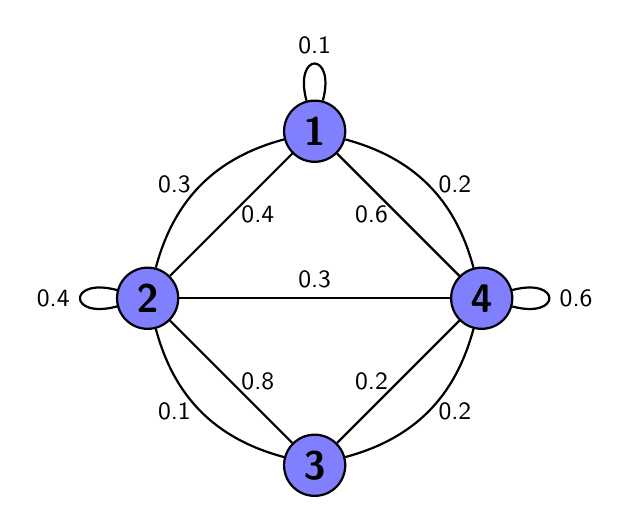
\begin{tikzpicture}[auto, node distance=3cm, every loop/.style={},
                    thick,main node/.style={circle,draw,fill=blue!50,font=\sffamily\Large\bfseries}]

  \node[main node] (1) {1};
  \node[main node] (2) [below left of=1] {2};
  \node[main node] (3) [below right of=2] {3};
  \node[main node] (4) [below right of=1] {4};

  \path[every node/.style={font=\sffamily\small}]
    (1) edge node [left] {0.6} (4)
        edge [bend right] node[left] {0.3} (2)
        edge [loop above] node {0.1} (1)
    (2) edge node [right] {0.4} (1)
        edge node {0.3} (4)
        edge [loop left] node {0.4} (2)
        edge [bend right] node[left] {0.1} (3)
    (3) edge node [right] {0.8} (2)
        edge [bend right] node[right] {0.2} (4)
    (4) edge node [left] {0.2} (3)
        edge [loop right] node {0.6} (4)
        edge [bend right] node[right] {0.2} (1);
\end{tikzpicture} The development of algorithms to handle graphs is therefore of major interest in computer science. The transformation of graphs is often formalized and represented by graph rewrite systems. Complementary to graph transformation systems focusing on rule-based in-memory manipulation of graphs are graph databases geared towards transaction-safe, persistent storing and querying of graph-structured data.
\subsection{{\color{blue} Linguistics:}}Graph-theoretic methods, in various forms, have proven particularly useful in linguistics, since natural language often lends itself well to discrete structure. Traditionally, syntax and compositional semantics follow tree-based structures, whose expressive power lies in the principle of compositionality, modeled in a hierarchical graph. More contemporary approaches such as head-driven phrase structure grammar model the syntax of natural language using typed feature structures, which are directed acyclic graphs. Within lexical semantics, especially as applied to computers, modeling word meaning is easier when a given word is understood in terms of related words; semantic networks are therefore important in computational linguistics. Still, other methods in phonology (e.g. optimality theory, which uses lattice graphs) and morphology (e.g. finite-state morphology, using finite-state transducers) are common in the analysis of language as a graph. Indeed, the usefulness of this area of mathematics to linguistics has borne organizations such as TextGraphs, as well as various 'Net' projects, such as WordNet, VerbNet, and others.
\subsection{{\color{blue}Physics and Chemistry:}}{\Huge \color{cyan}G}raph theory is also used to study molecules in {\color{green}\textit{Physics} } and  {\color{green}\textit{Chemistry} }. In condensed matter physics, the three-dimensional structure of complicated simulated atomic structures can be studied quantitatively by gathering statistics on graph-theoretic properties related to the topology of the atoms. Also, "the Feynman graphs and rules of calculation summarize quantum field theory in a form in close contact with the experimental numbers one wants to understand." In chemistry a graph makes a natural model for a molecule, where vertices represent atoms and edges bonds. This approach is especially used in computer processing of molecular structures, ranging from chemical editors to database searching. In statistical physics, graphs can represent local connections between interacting parts of a system, as well as the dynamics of a physical process on such systems. Similarly, in computational neuroscience graphs can be used to represent functional connections between brain areas that interact to give rise to various cognitive processes, where the vertices represent different areas of the brain and the edges represent the connections between those areas. Graph theory plays an important role in electrical modeling of electrical networks, here, weights are associated with resistance of the wire segments to obtain electrical properties of network structures.[13] Graphs are also used to represent the micro-scale channels of porous media, in which the vertices represent the pores and the edges represent the smaller channels connecting the pores. Chemical graph theory uses the molecular graph as a means to model molecules. Graphs and networks are excellent models to study and understand phase transitions and critical phenomena. Removal of nodes or edges lead to a critical transition where the network breaks into small clusters which is studied as a phase transition. This breakdown is studied via percolation theory.
\subsection{{\color{blue}Social sciences:}}

\begin{flushright}
{\Huge \color{cyan}G}raph theory is also widely used in sociology as a way, for example, to measure actors' prestige or to explore rumor spreading, notably through the use of social network analysis software. Under the umbrella of social networks are many different types of graphs.\includegraphics[height=4cm]{C:/Users/User/Pictures/Sociology.jpg}Acquaintanceship and friendship graphs describe whether people know each other. Influence graphs model whether certain people can influence the behavior of others. Finally, collaboration graphs model whether two people work together in a particular way, such as acting in a movie together.
\\

\end{flushright}
 

\end{document}